\begin{figure}[ht!]
\centering
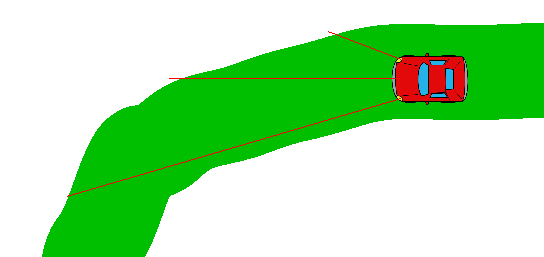
\includegraphics[width=65mm]{data/car1.png}
\caption{Els sensors detecten la distància del cotxe a les parets del circuit.}
\label{sensors}
\end{figure}

La nostra segona demostració és radicalment diferent a la primera:
l'objectiu és programar un automòbil el qual, a partir de tres sensors frontals,
sigui capaç d'evitar xocar amb les parets de \emph{qualsevol circuit}.
És a dir; el seu entrenament ha de ser general i adaptable a qualsevol situació.

Per a solucionar un problema com aquest, no disposem d'un \emph{dataset},
com en el cas del reconeixement de caràcters: qui s'ha dedicat a crear
una base de dades que representa totes les decisions que hauria de prendre
el cotxe, en qualsevol dels casos en que es pot trobar? Evidentment, no és
una tàctica adequada.

Hem d'atacar el problema des d'un altre punt de vista: ara ja no es tracta
d'una situació en la qual l'entrenament de l'agent es pugui supervisar
(\emph{supervised learning}), ara ha d'ésser ell mateix qui explori l'entorn
en el qual es troba. Utilitzarem el segon mètode més popular d'aprenentatge
de màquina: l'aprenentatge sense supervisió (\emph{unsupervised learning}, o \emph{reinforcement learning}).
\\

\section{Reinforcement Learning}

\begin{figure}[ht!]
\centering
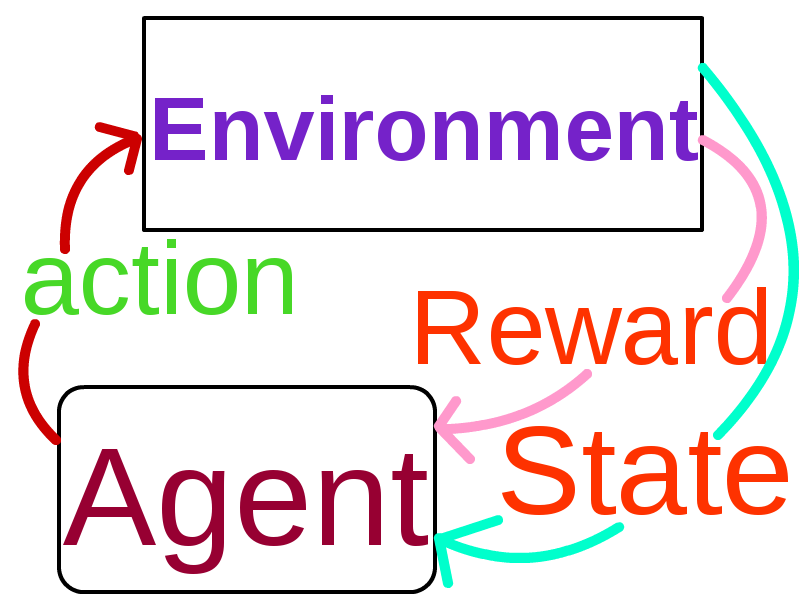
\includegraphics[width=52mm]{data/reinforce.png}
\caption{Diagrama que representa l'aprenentatge per reforç.}
\label{reinforcegraph}
\end{figure}

L'\emph{aprenentatge per reforç} es basa en la presa de decisions de l'agent en base
a una prèvia exploració de l'entorn, la qual ha sigut controlada a través d'un sistema
de recompenses \cite{reinflnbk}.

Ho podem il·lustrar de forma senzilla: un ratolí representa el nostre agent. Aquest divaga
de forma aleatòria a través d'un entorn desconegut. Quan cau a una trampa, se li dona una
recompensa negativa; quan es troba amb un tros de formatge, una de positiva. Poc a poc,
el ratolí aprendrà a evitar trampes i buscar el formatge.

Expressat amb termes més tècnics: el ratolí es troba en un estat \(s\) (que
emmagatzema la quantitat de peces de formatge que té, i si està viu o no), i
realitza una acció \(a\). Això el porta a trobar-se en un estat \(s'\).
Es fa llavors una comparació entre els dos estats, \(s\) i \(s'\), i se
li dona una recompensa \(r\) en base a uns criteris (per cada tros de formatge
que hagi guanyat, \(+5\); si segueix viu, \(+1\); si ha caigut en una trampa,
\(-100\)).

Aquesta és l'essència
de l'aprenentatge per reforç.

\section{Q-Learning}

\emph{Q-learning} és un algoritme d'aprenentatge per esforç. Expressat de forma
matemàtica:

\[
Q[s, a] = Q[s, a] + \alpha(r + \lambda V(s') - Q[s, a])
\]

Però que no espanti massa. En realitat, és extremadament fàcil d'implementar (en 
comparació a l'ús d'una \ac{ann}; no hem ni escrit les fórmules adients, degut a la seva
complexitat). Anem pas per pas, seguint el camí que hem fet per a arribar a 
un programa funcional.

Primer de tot, hem de mesurar l'estat en que es troba el nostre agent. Aquesta mesura ha de tenir les dades
que siguin necessàries per a corregir l'agent. Ens interessa, principalment, la distància
a les parets del circuit. Per a fer-ho efectivament, hem projectat tres \emph{làsers} o
sensors, que s'allarguen fins que el color sobre el qual es troben no és el color del circuit.
Un làser va en direcció igual a la del cotxe, i els altres dos es desvien 15 graus per a obtenir
una visió panoràmica de la posició del vehicle \ref{sensors}. Dibuixar les línies que
representen els sensors ha sigut tot un repte en quant a programació i matemàtiques.

Ara ja podem calcular la llargada dels làsers; és això tot el que necessitem per mesurar l'estat
en que es troba el vehicle, i donar-li una recompensa. Però, l'algoritme \emph{Q-learning} té una limitació: la seva aplicació
comporta la creació d'un \emph{array} \footnote{També conegut com a \emph{vector}: llista de valors}
que tindrà una quantitat d'entrades igual a \emph{totes les possibles combinacions d'estat}. És a dir,
en el cas dels sensors del cotxe, que poden arribar a tenir un valor de 1,000 (píxels), l'array
tindrà \num{1000000000} entrades (1000 valors possibles per sensor, multiplicat per sí mateix tres vegades, la quantitat
de sensors que tenim). No és viable; hem de \emph{discretitzar} una magnitud que, a efectes pràctics, és contínua.

Per tant, volem convertir el valor del sensor a una categoria del 0 al 9, on 0 significa ``molt a prop'', i 9 ``molt lluny'',
per a poder crear un array de dimensions viables (en aquest cas, tenim 10 estats per sensor, per tant, 1000 estats en total).
Com que ens interessa entrenar amb més precisió els casos en que els sensors tenen distàncies molt curtes (el cotxe està a 
prop de la paret), ens agradaria transformar de forma no simètrica els valors dels sensors, és a dir, que un valor real de
250px es transformi a 5, per exemple, i no a 2.5
Primer vam intentar realitzar aquest procés de discretització a partir d'una transformació logarítmica:
\[
s_i(D) = \left\lfloor 9 \frac{ln(D)}{ln(1000)} \right\rfloor
\]
però els valors resultants estaven massa desproporcionats. Vam decidir fer-ho a la força bruta, establint condicions
simples. 

Solucionat el problema dels estats.














